%versi 2 (8-10-2016)
\chapter{Dasar Teori}
\label{chap:teori}

Bab dua ini berisi dasar-dasar teori yang terkait dengan BPM, BPMN, BPMS, dan sistem email

\section{\textit{Business Process} (BP)}
\label{sec:bp}
\textit{Business Process} adalah kumpulan dari \textit{event}/kejadian, \textit{activity}/kegiatan, dan \textit{decision point}/keputusan serta melibatkan sejumlah aktor dan objek yang bertujuan untuk menghasilkan nilai dalam bentuk produk/jasa yang berguna bagi konsumen\cite{dumas:13} .

\subsection{Komponen \textit{Business Process}}
\label{sec:komponenBP}
\textit{Business Process Management} memiliki komponen-komponen sebagai berikut :
\begin{description}
	\item{\textit{Event}} \hfill \\\textit{Event} adalah kejadian yang terjadi saat proses bisnis berjalan. 
	\item{\textit{Activity}} \hfill \\\textit{Activity} adalah kumpulan kegiatan yang dapat dikerjakan. Ketika suatu \textit{Activity} berupa sebuah kegiatan yang sederhana, \textit{activity} disebut dengan \textit{task}. 
	\item{\textit{Decision Point}} \hfill \\\textit{Decision point} adalah keputusan yang mempengaruhi proses selanjutnya.
	\item{\textit{Actor}} \hfill \\ \textit{Actor} berupa individu, organisasi, maupun sistem yang mempengaruhi proses bisnis. 
	\item{\textit{Object}} \hfill \\ \textit{Object} dapat berupa objek fisik (peralatan, bahan baku, produk, dokumen) maupun non fisik (dokumen elektronik, basis data elektronik).
	\item{\textit{Positive/Negative Outcome}} \hfill \\ Hasil dari bisnis proses dapat menghasilkan nilai bagi konsumen (positif) atau tidak menghasilkan nilai (negatif).
\end{description}
Komponen-komponen penyusun proses bisnis dapat dilihat pada Gambar ~\ref{komponenbp}.
\begin{figure}[H]
	\centering
	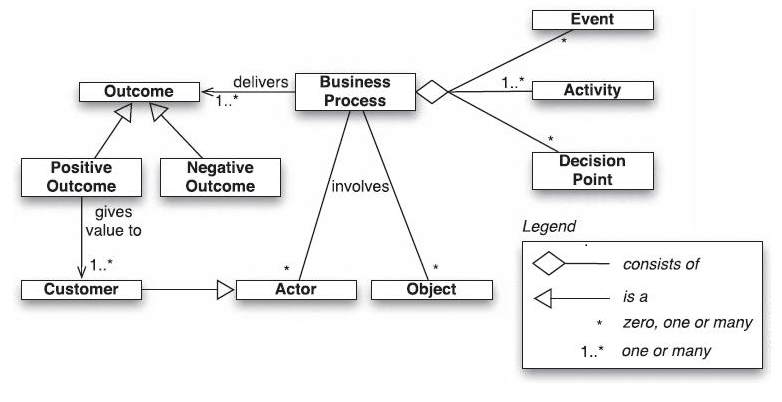
\includegraphics[scale=0.7]{Gambar/Bab-2/1-bp-components}
	\caption{Komponen BPM} 
	\label{komponenbp}
\end{figure}





\section{\textit{Business Process Management}(BPM)}
\label{sec:bpm}
\textit{Business Process Management} merupakan kumpulan metode, teknik, dan alat untuk menemukan, menganalisa, mendesain kembali, menjalankan, dan mengawasi proses bisnis. 
\subsection{Siklus \textit{Business Process Management}}
\label{sec:siklusBPM}
Suatu proses bisnis tidak selalu berjalan dengan baik. Banyak hal yang tidak diantisipasi sebelumnya dapat menggangu proses bisnis. Untuk menjaga kualitas dari sebuah proses bisnis diperlukan pengawasan dan kontrol pada suatu fase tertentu serta perbaikan apabila diperlukan. Maka dari itu, suatu bisnis proses dapat dilihat sebagai suatu siklus yang terus menerus meningkatkan kualitasnya. Siklus dalam proses bisnis berupa :

\begin{description}
	\item{\textit{Process Identification}} \hfill \\ Pada fase ini, suatu masalah bisnis ditemukan, kemudian proses-proses yang berhubungan dengan masalah bisnis tersebut diidentifikasi, dibatasi, dan dihubungkan satu sama lain. Proses ini terbagi menjadi dua tahap, yaitu \textit{designation} dan \textit{evaluation}. Tahap \textit{designation} bertujuan untuk mengenali proses-proses yang ada dan hubungan antar proses tersebut. Sedangkan tahap \textit{evaluation} memprioritaskan proses-proses yang menghasilkan nilai dan mempertimbangkan proses yang memiliki risiko atau tidak menghasilkan nilai. Fase ini menghasilkan arsitektur dari proses bisnis yang merepresentasikan proses bisnis dan relasi-relasinya.   
	\item{\textit{Process Discovery}} \hfill \\ Setiap proses yang relevan dengan masalah bisnis didokumentasikan, umumnya dalam bentuk model proses. Fase ini menghasilkan \textit{as-is process model}
	\item{\textit{Process Analysis}} \hfill \\ Pada fase ini, masalah pada model proses diidentifikasi, didokumentasikan, dan diukur kinerjanya dengan ukuran yang telah ditetapkan. Hasil dari fase ini adalah kumpulan masalah pada proses model.
	\item{\textit{Process Redesign}} \hfill \\ Tujuan dari fase ini adalah membuat perubahan pada proses yang dapat mengatasi berbagai kumpulan masalah yang telah diidentifikasi pada fase sebelumnya. Proses ini menghasilkan \textit{to-be process model}.
	\item{\textit{Process Implementation}} \hfill \\ Pada fase ini, model proses diimplementasikan untuk diekseskusi menggunakan \textit{Business Process Management System}.
	\item{\textit{Process Monitoring and Controlling}} \hfill \\ Setelah proses bisnis berjalan pada BPMS, berbagai data yang relevan dikumpulkan dan dianalisa untuk menentukan kualitas dari proses. Apabila terdapat masalah baru yang ditemukan, maka proses diulangi.
\end{description}
Siklus BPM dapat dilihat pada Gambar ~\ref{siklusbpm}.
\begin{figure}[H]
	\centering
	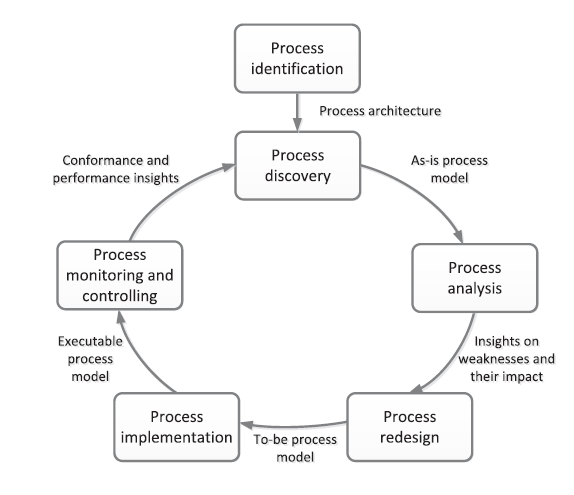
\includegraphics[scale=0.7]{Gambar/Bab-2/2-bpm-lifeCycle}
	\caption{Siklus BPM} 
	\label{siklusbpm}
\end{figure}


\section{\textit{Business Process Model and Notation}}
\label{sec:bpmn}
Business Process Model Notation (BPMN) adalah notasi grafis yang menggambarkan langkah-langkah dalam proses bisnis\cite{bpmn:15:camunda}. Notasi-notasi tersebut terdiri dari \textit{Event}, \textit{Activity}, \textit{Gateway}, \textit{Data}, \textit{Artifact}, \textit{Pools}, dan \textit{Lanes}.

\subsection{\textit{Event}}
\label{sec:event}
Event merupakan kejadian yang terjadi pada proses bisnis yang dilambangkan dengan bentuk lingkaran. Notasi event secara umum terbagi menjadi tiga, yaitu \textit{start event, intermediate event,} dan \textit{end event}. \textit{Start event} menunjukkan dimulainya proses, \textit{intermediate event} dapat muncul ketika proses berjalan, sedangkan \textit{end event} menunjukkan berakhirnya proses.  
\begin{figure}[H]
	\centering
	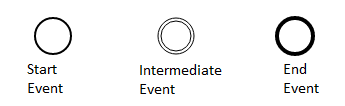
\includegraphics[scale=1]{Gambar/Bab-2/bpmn/event1}
	\caption{Notasi \textit{Event}} 
	\label{event}
\end{figure}

\subsection{\textit{Activity}}
\label{sec:activity}
\textit{Activity} merupakan kumpulan kegiatan yang dapat dikerjakan. Sebuah \textit{task} merupakan bagian dari \textit{Activity} yang tidak dapat dipecah lagi. Bebera jenis dari \textit{Task} adalah :
	\begin{enumerate}
		\item{\textit{User Task}}, yaitu pekerjaan yang perlu dilakukan oleh manusia melalui sistem. Contohnya adalah mengisi formulir pada halaman web, mengganti password.
		\item{\textit{Manual Task}}, yaitu pekerjaan yang dilakukan manusia tanpa melalui sistem. Contohnya adalah mengirim barang, mengirim surat.
		\item{\textit{Service Task}}, yaitu pekerjaan yang dilakukan oleh sistem dengan mengeksekusi kode. Contohnya adalah notifikasi dari sistem, membangkitkan nomor token. 
	\end{enumerate}
	
	
\begin{figure}[H]
	\centering
	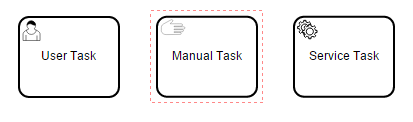
\includegraphics[scale=1]{Gambar/Bab-2/bpmn/task}
	\caption{Notasi \textit{Task}} 
	\label{task}
\end{figure}

\subsection{\textit{Gateway}}
\label{sec:gateway}
\textit{Gateway} merupakan simbol yang menentukan percabangan dan penggabungan jalur dalam proses. Gateway dilambangakan dengan belah ketupat. Beberapa macam adalah :
\begin{itemize}
	\item \textit{Exclusive Gateway} (XOR) berarti memilih salah satu dari cabang yang ada. 
	\item \textit{Inclusive Gateway} berarti memilih satu, beberapa, atau seluruh cabang yang ada.
	\item \textit{Parallel Gateway} berarti mengerjakan proses pada seluruh cabang yang ada.
	\item \textit{Event Based} berarti mengerjakan proses setelah suatu \textit{event} selesai.
\end{itemize} 

\begin{figure}[H]
	\centering
	
\includegraphics[scale=1]{Gambar/Bab-2/bpmn/gateway}
	\caption{Notasi \textit{Gateway}} 
	\label{gateway}
\end{figure}


%\subsection{\textit{Flow}}
%\label{sec:flow}

%\begin{figure}[H]
%	\centering
%	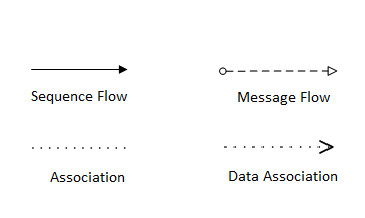
\includegraphics[scale=1]{Gambar/Bab-2/bpmn/flow}
%	\caption{Notasi \textit{Flow}} 
%	\label{flow}
%\end{figure}

\subsection{\textit{Data}}
\label{sec:data}
\textit{Data Object} melambangkan informasi yang berjalan dalam proses seperti dokumen, e-mail, atau surat. Sedangkan \textit{Data Store} merupakan tempat proses membaca atau menyimpan data seperti basis data atau rak. 
\begin{figure}[H]
	\centering
	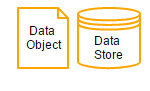
\includegraphics[scale=1]{Gambar/Bab-2/bpmn/data}
	\caption{Notasi \textit{Data}} 
	\label{data}
\end{figure}


\subsection{\textit{Artifact}}
\label{sec:artifacts}
\textit{Artifact} tidak mempengaruhi jalannya proses, tetapi hanya sebagai informasi tambahan agar proses lebih mudah dimengerti. Terdapat dua jenis, yaitu \textit{Text Annotation} dan \textit{Group}
\begin{figure}[H]
	\centering
	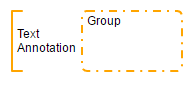
\includegraphics[scale=1]{Gambar/Bab-2/bpmn/artifact}
	\caption{Notasi \textit{Artifact} }
	\label{artifact}
\end{figure}


\subsection{\textit{Pools} dan \textit{Lanes}}
\label{sec:poolslanes}
\textit{Lanes} digunakan untuk memberikan kumpulan \textit{tasks} kepada yang bertanggung jawab untuk mengerjakannya. Sedangkan \textit{Pools} merupakan kumpulan dari \textit{Lanes}.
\begin{figure}[H]
	\centering
	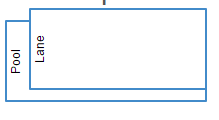
\includegraphics[scale=1]{Gambar/Bab-2/bpmn/swimlane}
	\caption{Notasi \textit{Lanes dan Pools}} 
	\label{lanespools}
\end{figure}


 

\section{\textit{Business Process Management System (BPMS)}}
\textit{Business Process Management System (BPMS)} adalah sistem yang mengkoordinasikan otomatisasi proses bisnis. Tujuan dari BPMS adalah menyelesaikan proses pada waktu yang ditentukan dan menggunakan sumber daya yang tepat. 

Arsitektur BPMS
Komponen-komponen BPMS beserta hubungannya yang ditunjukkan pada Gambar ~\ref{fig:arsitekturbpms} terdiri dari :
\begin{itemize}
	\item \textit{Execution Engine}, menyediakan beberapa fungsi seperti mengeksekusi proses, mendistribusikan \textit{task}, mengambil dan menyimpan data yang diperlukan. 
	\item \textit{Process Modeling Tool}, \textit{tool} untuk membuat model proses.
	\item \textit{Worklist Handler}, \textit{tool} untuk mendistribusikan pekerjaan.
	\item \textit{Administration dan Monitoring Tool} \textit{tools} untuk administrasi dan memonitor proses. 
	%\item \textit{Repository}
	%\item \textit{Execution Logs}
\end{itemize}
\begin{figure}[H]
	\centering
	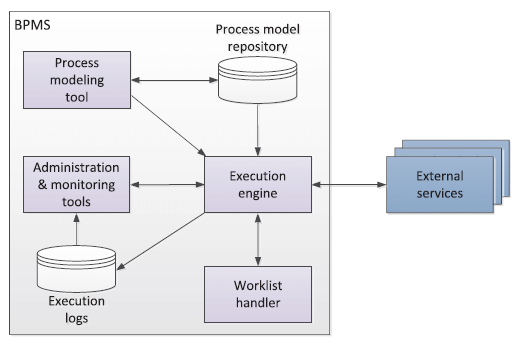
\includegraphics[scale=0.7]{Gambar/Bab-2/bpms/bpms}
	\caption{Arsitektur BPMS} 
	\label{fig:arsitekturbpms}
\end{figure}



\section{BPMS Camunda}
\label{bpmscamunda}
Camunda adalah \textit{framework} BPMS berbasis Java yang mendukung \textit{workflow} BPMN dan otomatisasi proses bisnis\cite{bpmmanual:15:7.6}. 

\subsection{Arsitektur BPMS Camunda}
\label{arsitekturcamunda}
Komponen-komponen pada BPMS Camunda adalah sebagai berikut :
\begin{figure}[H]
	\centering
	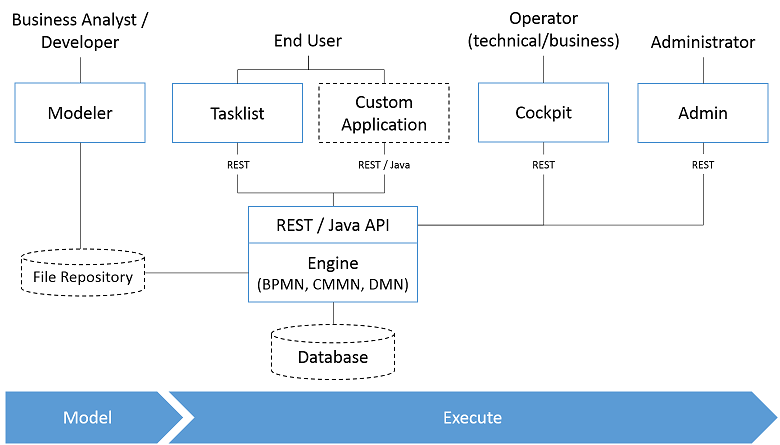
\includegraphics[scale=0.7]{Gambar/Bab-2/bpms/arsitektur-camunda}
	\caption{Arsitektur BPMS Camunda} 
	\label{fig:arsitekturcamunda}
\end{figure}

\begin{itemize}
	\item \textit{Modeler}, \textit{tool} untuk membuat diagram BPMN yang dapat dieksekusi. Camunda Modeler menyediakan berbagai notasi yang diperlukan untuk membuat diagram BPMN. Terdapat pula beberapa pengaturan yang dapat dimasukkan ke dalam notasi.
		\begin{figure}[H]
			\centering
			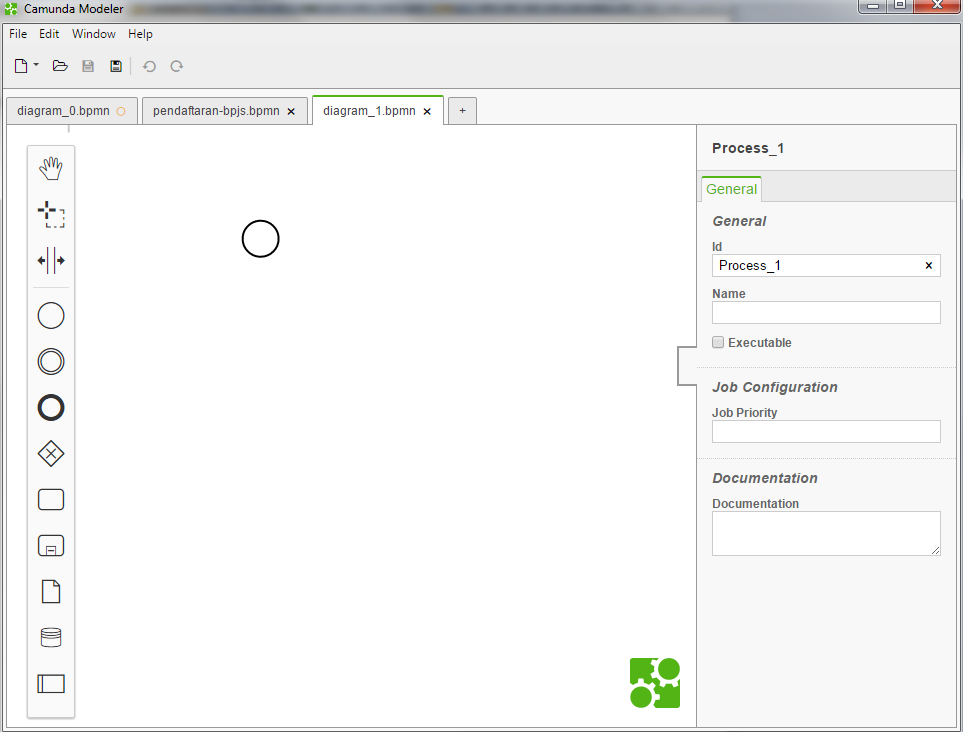
\includegraphics[scale=0.4]{Gambar/Bab-2/bpms/camundaModeler}
			\caption{Camunda Modeler} 
			\label{fig:camundamodeler}
		\end{figure}
	
		Terdapat tiga bagian utama pada Camunda Modeler, yaitu :
\begin{enumerate}
	\item Bagian kiri merupakan kumpulan \textit{tool} dan notasi untuk membuat diagram BPMN.
	\item Bagian tengah merupakan tempat membuat diagram BPMN.
	\item Bagian kanan merupakan pengaturan untuk tiap \textit{event}, \textit{task}, maupun notasi lainnya. Berikut ini adalah penjelasan untuk beberapa kolom pengaturan \textit{user task} :
	\begin{enumerate}
		\item Tab General
			\begin{itemize}
				\item Id, yaitu id dari \textit{task}
				\item Name, yaitu nama dari \textit{task}
				\item Assignee, yaitu nama pemilik \textit{task}
				\item Candidate Users, yaitu kandidat pemilik dari \textit{task}
				\item Candidate Group, yaitu kandidat grup dari \textit{task}
				\item Due Date, yaitu pengaturan batas waktu
				\item Follow Up Date, yaitu pengaturan waktu \textit{follow up}
			\end{itemize}
			\begin{figure}[H]
				\centering
				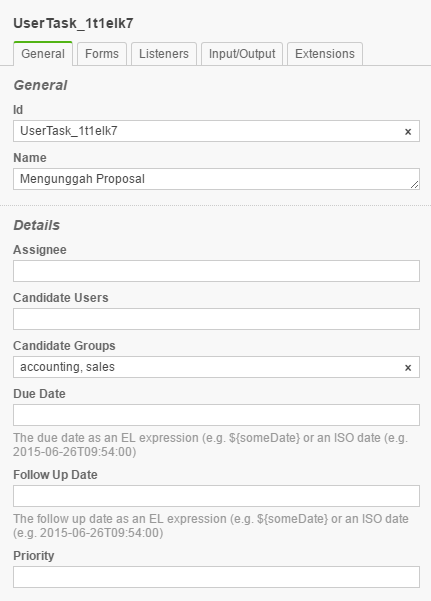
\includegraphics[scale=0.5]{Gambar/Bab-3/Modeler/3Properties}
				\caption{Tampilan Pengaturan Camunda Modeler} 
				\label{fig:camundaModelerPropertiesGeneral}
			\end{figure}
		\item Tab Forms, tempat untuk mengisi lokasi halaman web yang diacu oleh \textit{user task}
		\begin{figure}[H]
				\centering
				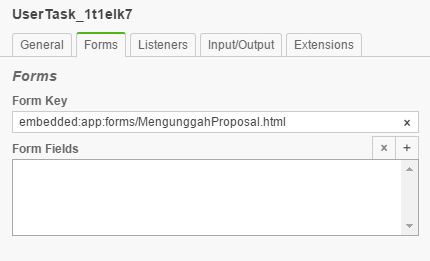
\includegraphics[scale=0.5]{Gambar/Bab-3/Modeler/4}
				\caption{Tampilan Pengaturan Camunda Modeler} 
				\label{fig:camundaModelerPropertiesForms}
		\end{figure}
		\item Listener, terbagi menjadi dua, yaitu \textit{Execution Listener} dan \textit{Task Listener}. Listener berfungsi untuk menjalankan perintah ketika ada suatu \textit{event} yang terjadi. Misalnya \textit{Task Listener} dengan event \textit{create} akan dijalankan ketika \textit{task} dibuat.
		\begin{figure}[H]
				\centering
				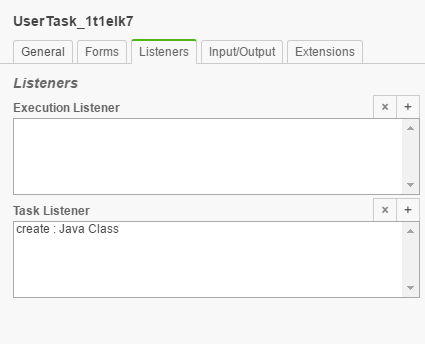
\includegraphics[scale=0.5]{Gambar/Bab-3/Modeler/5}
				\caption{Tampilan Pengaturan Camunda Modeler} 
				\label{fig:camundaModelerPropertiesListener}
		\end{figure}
	\end{enumerate}		




\end{enumerate}
	
	\item \textit{Tasklist}, tempat pengguna mengakses dan mengerjakan tugas. Tugas yang dikerjakan mengikuti alur model proses (BPMN) yang telah dibuat. 
		\begin{figure}[H]
			\centering
			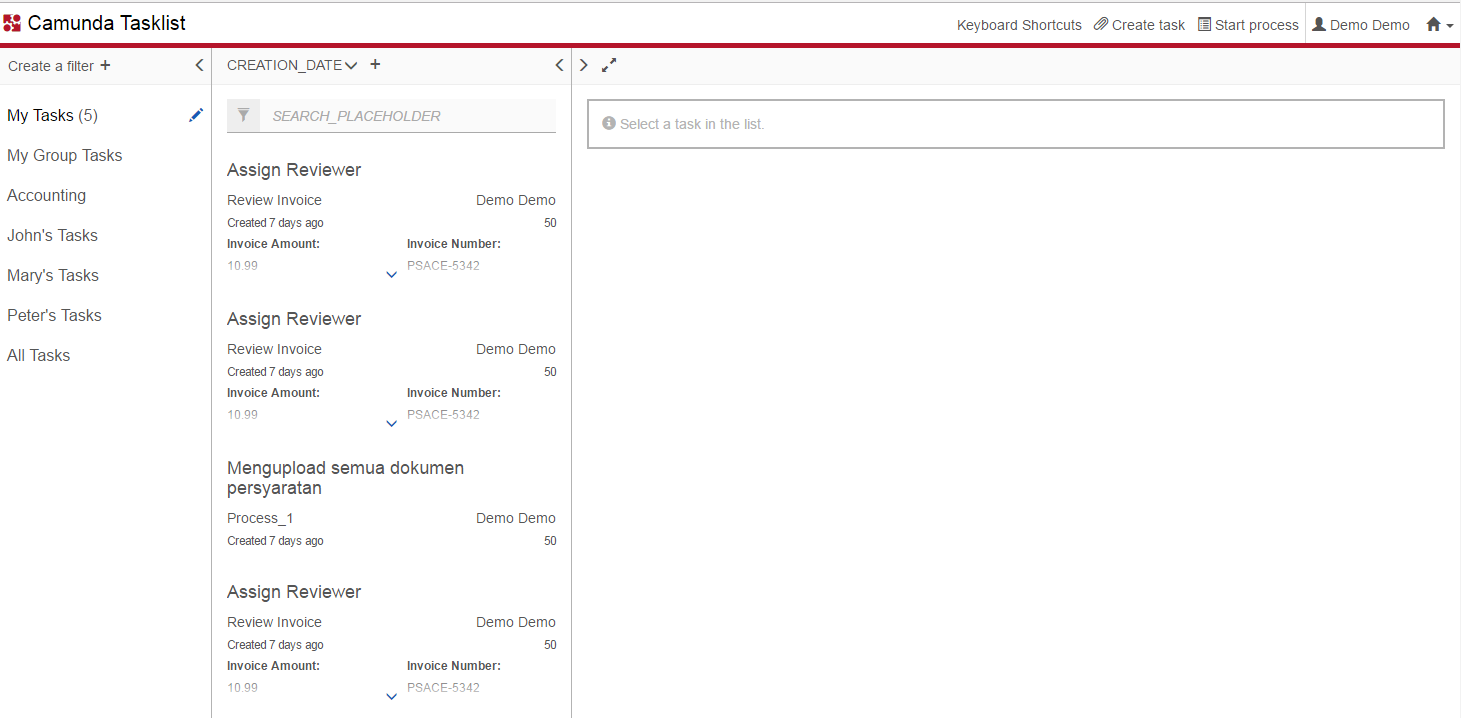
\includegraphics[scale=0.4]{Gambar/Bab-2/bpms/camundaTaskList}
			\caption{Camunda Tasklist} 
			\label{fig:camundatasklist}
		\end{figure}
	
	\item \textit{Cockpit}, memeriksa proses yang sedang berjalan maupun proses yang sudah selesai.
	\begin{figure}[H]
	\centering
	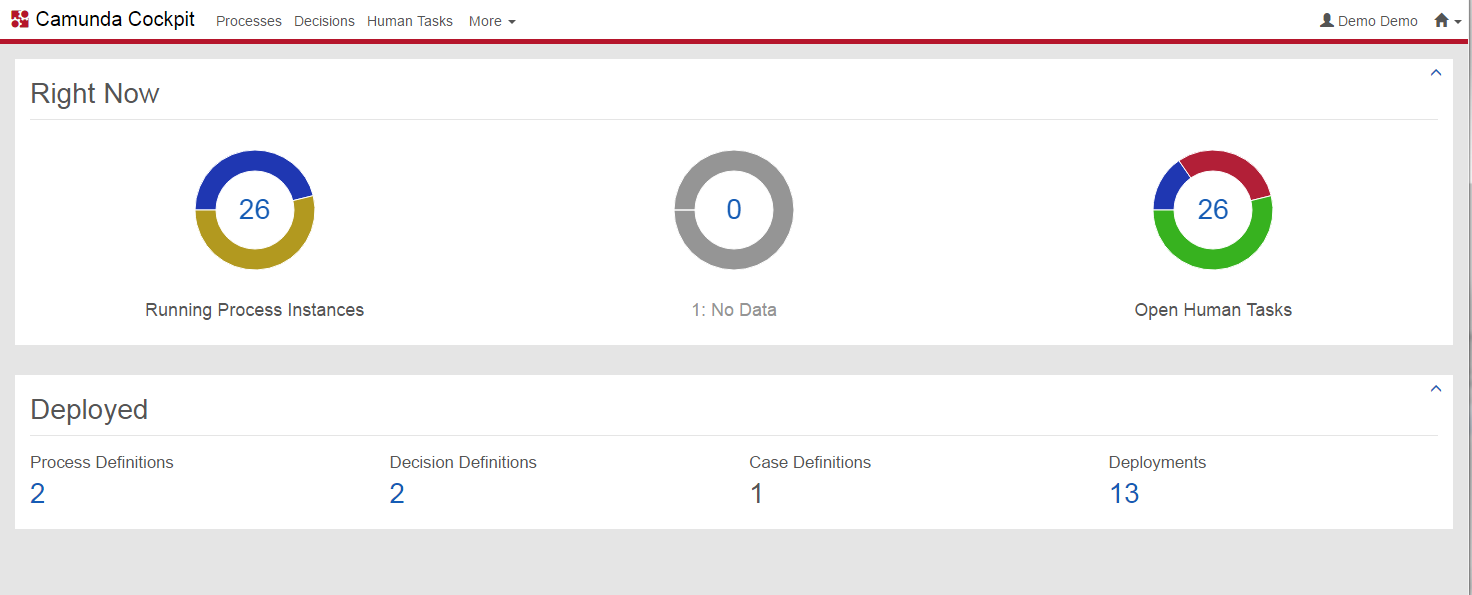
\includegraphics[scale=0.4]{Gambar/Bab-2/bpms/camundaCockpit}
	\caption{Camunda Cockpit} 
	\label{fig:camundacockpit}
\end{figure}
	
\item \textit{Admin}, memiliki tugas untuk mengatur, mengelompokkan, dan memberi izin kepada pengguna untuk melakukan tugas.
	\begin{figure}[H]
	\centering
	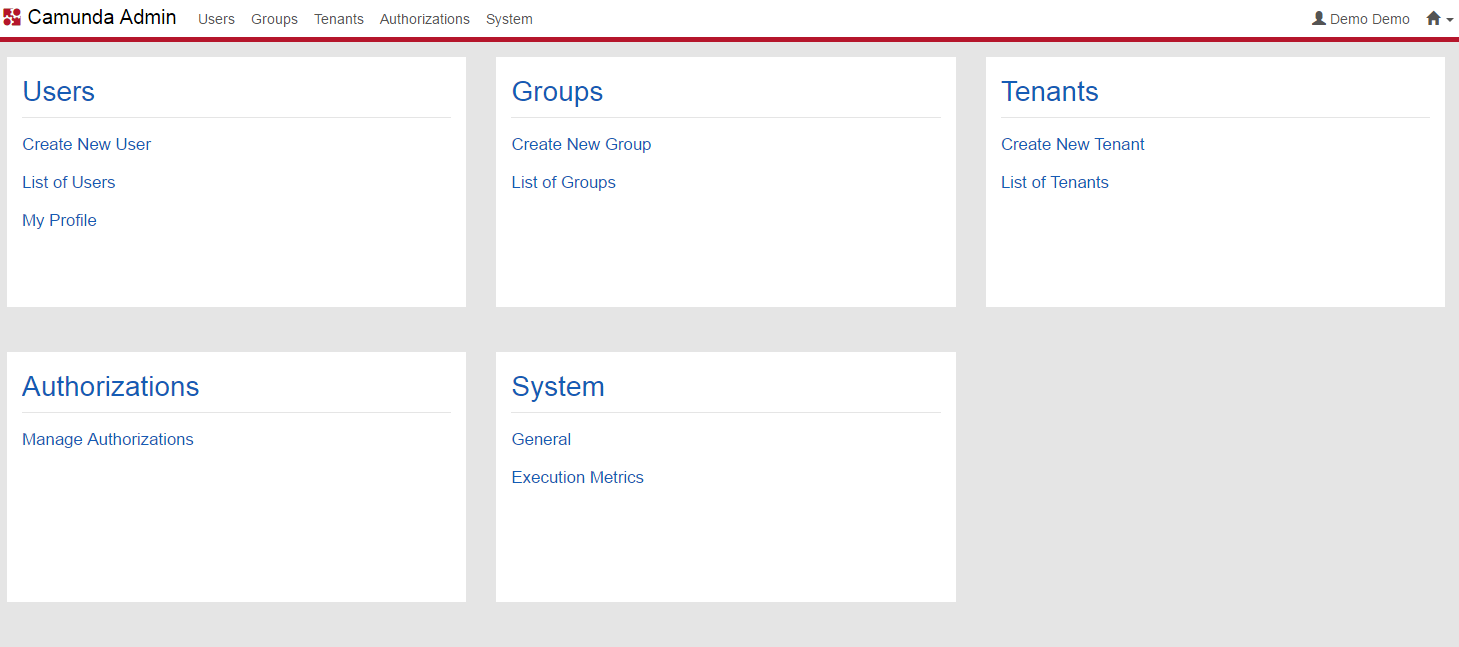
\includegraphics[scale=0.4]{Gambar/Bab-2/bpms/camundaAdmin}
	\caption{Camunda Admin} 
	\label{fig:camundaadmin}
\end{figure}

	\item \textit{Custom Application}, aplikasi lain yang diintegrasikan dengan Camunda menggunakan Java atau REST API.
	
\end{itemize}

\section{Forms SDK}
\label{formssdk}
Camunda menggunakan Forms SDK untuk mengimplementasikan \textit{user task} menggunakan aplikasi berbasis HTML5 / JavaScript. Forms SDK menyediakan instruksi untuk mengakses variabel proses pada \textit{form} HTML. Terdapat dua tipe instruksi yaitu cam-variable-name yang digunakan untuk memberi nama proses / \textit{task} / variabel dan cam-variable-type yang digunakan untuk mementukan tipe dari variabel. Elemen HTML yang didukung adalah :
\begin{enumerate}
	\item \textit{Text Inputs}, untuk memasukkan satu baris teks dan dapat diisi dengan berbagai tipe data seperti String, Integer, Long, Short, dan Double. Kodenya sebagai berikut:
		\begin{lstlisting}[language=html,basicstyle=\tiny,caption=Text Input]
			<input type="text" cam-variable-name="CUSTOMER_ID" cam-variable-type="String" />
		\end{lstlisting}
		
	\item \textit{Text Areas}, untuk memasukkan teks dan dapat diisi dengan berbagai tipe data seperti String, Integer, Long, Short, dan Double. Kodenya sebagai berikut:
		\begin{lstlisting}[language=html,basicstyle=\tiny,caption=Text Areas]
			<textarea cam-variable-name="CUSTOMER_ADDRESS" cam-variable-type="String"></textarea>
		\end{lstlisting}
			
	\item \textit{Date Inputs}, untuk memasukkan tanggal dengan format yyyy-MM-dd'T'HH:mm:ss (contoh:2017-05-30T11:00:00). Kodenya sebagai berikut:
		\begin{lstlisting}[language=html,basicstyle=\tiny,caption=Date Inputs]
			<input type="text"
       cam-variable-name="CONTRACT_START_DATE"
       cam-variable-type="Date" />
		\end{lstlisting}		


	\item \textit{Boolean Inputs}, terdiri dari tiga tipe, yaitu Checkbox, Select Box, dan Text Inputs (pengguna harus menulis \textit{true} atau \textit{false}. Kodenya sebagai berikut :
	\begin{lstlisting}[language=html,basicstyle=\tiny,caption=Boolean Inputs]

	<input type="checkbox"cam-variable-name="IS_VIP_CUSTOMER"cam-variable-type="Boolean" /> 
	
	<select cam-variable-name="APPROVED" cam-variable-type="Boolean">
		<option value="true">Yes</option>
		<option value="false">No</option>
	</select>
	
	<input type="text"cam-variable-name="IS_VIP_CUSTOMER"cam-variable-type="Boolean" />
	\end{lstlisting}
	
	
	\item \textit{Selects}, untuk memilih salah satu pilihan. Kodenya sebagai berikut :
	\begin{lstlisting}[language=html,basicstyle=\tiny,caption=Selects]
	<select cam-variable-name="foo"
        cam-variable-type="String">
  <option>bar</option>
  <option>zar</option>
</select>
\end{lstlisting}

	\item \textit{Hidden Input Fields}, untuk menyembunyikan \textit{form}. Kodenya sebagai berikut :
	\begin{lstlisting}[language=html,basicstyle=\tiny,caption=Hidden Input Fields]
	<input type="hidden"
       cam-variable-name="CUSTOMER_ID"
       cam-variable-type="String"
       value="testuser" />
	\end{lstlisting}
	
	\item \textit{Upload} dan \textit{Download}, untuk mengunggah maupun mengunduh file. Kode untuk mengunggah file sebagai berikut :
		\begin{lstlisting}[language=html,basicstyle=\tiny,caption=Upload]
	<input type="file"
       cam-variable-name="INVOICE_DOCUMENT"
       cam-variable-type="File"
       cam-max-filesize="10000000" />
	\end{lstlisting}
Sedangkan kode untuk mengunduh file sebagai berikut :
\begin{lstlisting}[language=html,basicstyle=\tiny,caption=Download]
<a cam-file-download="INVOICE_DOCUMENT"></a>
\end{lstlisting}

Nama variabel pada cam-variable-name harus sama dengan nama variabel pada cam-file-download.

	\end{enumerate}

\section{Email}
\label{email}

\subsection{Mail Server}
\label{servermail}
\textit{Mail server} adalah mekanisme pengiriman email yang menyediakan berbagai standar sehingga email bisa dikirim dari satu domain ke domain lainnya. \textit{Mail server} dapat dikategorikan menjadi dua, yaitu :
\begin{enumerate}
	\item \textit{Mail server} yang menuju ke dalam, yaitu  server SMTP \textit{Simple Mail Transfer Protocol}. Protokol SMTP digunakan untuk mengirim email dari sebuah klien ke alamat yang dituju.
	\item \textit{Mail server} yang menuju ke luar, yaitu server POP3 \textit{Post Office Protocol} dan server IMAP \textit{Internet Message Access Protocol}.

\end{enumerate}

\subsection{JavaMail}
\label{javamail}
JavaMail adalah Java API yang digunakan untuk mengirim dan menerima email melalui SMTP (Simple Mail Transfer Protocol), POP3 (Post Office Protocol 3), dan IMAP (Internet Message Access Protocol)\cite{javamail}. JavaMail dibuat dalam lingkungan Java Enterprise Edition (Java EE) yang merupakan lingkungan komputasi untuk pengembangan perangkat lunak skala besar dan menggunakan jaringan yang aman.


Untuk menggunakan JavaMail diperlukan beberapa kelas, yaitu :
\begin{itemize}
	\item Kelas Session, kelas untuk mengumpulkan atribut email yang akan digunakan. Kelas Session mengambil berbagai atribut dari kelas Properties, seperti informasi server email yang akan digunakan.
	\item Kelas MimeMessage, kelas untuk menulis email. Kelas ini menyediakan berbagai atribut untuk menulis email. Di antaranya adalah alamat email asal, alamat email penerima, subjek, isi email, dll.
	\item Kelas Transport, kelas untuk membuat koneksi ke email \textit{server} dan mengirim email.
\end{itemize}
Di bawah ini adalah contoh kode pengiriman email menggunakan JavaMail API : 
\begin{lstlisting}[language=Java,basicstyle=\tiny,caption=Contoh Kode Pengiriman Email]
Properties props = new Properties();
    props.put("mail.smtp.host", "my-mail-server");
    Session session = Session.getInstance(props, null);

    try {
        MimeMessage msg = new MimeMessage(session);
        msg.setFrom("me@example.com");
        msg.setRecipients(Message.RecipientType.TO,
                          "you@example.com");
        msg.setSubject("JavaMail hello world example");
        msg.setSentDate(new Date());
        msg.setText("Hello, world!\n");
        Transport.send(msg, "me@example.com", "my-password");
    } catch (MessagingException mex) {
        System.out.println("send failed, exception: " + mex);
    }
		
\end{lstlisting}


 %
%\subsection{Kutipan}
%\label{subs:kutipan} 
%Berikut contoh kutipan dari berbagai sumber, untuk keterangan lebih lengkap, silahkan membaca file referensi.bib yang disediakan juga di template ini.
%Contoh kutipan:
%\begin{itemize}
	%\item Buku:~\cite{berg:08:compgeom} 
	%\item Bab dalam buku:~\cite{kreveld:04:GIS}
	%\item Artikel dari Jurnal:~\cite{buchin:13:median}
	%\item Artikel dari prosiding seminar/konferensi:~\cite{kreveld:11:median}
	%\item Skripsi/Thesis/Disertasi:~\cite{lionov:02:animasi}~\cite{wiratma:10:following}~\cite{wiratma:22:later}
	%\item Technical/Scientific Report:~\cite{kreveld:07:watertight}
	%\item RFC (Request For Comments):~\cite{RFC1654}
	%\item Technical Documentation/Technical Manual:~\cite{Z.500}~\cite{unicode:16:stdv9}~\cite{google:16:and7}
	%\item Paten:~\cite{webb:12:comm}
	%\item Tidak dipublikasikan:~\cite{wiratma:09:median}~\cite{lionov:11:cpoly}
	%\item Laman web:~\cite{erickson:03:cgmodel}  
	%\item Lain-lain:~\cite{agung:12:tango}
%\end{itemize}    
  %
%\subsection{Gambar}
%
%Pada hampir semua editor, penempatan gambar di dalam dokumen \LaTeX{} tidak dapat dilakukan melalui proses {\it drag and drop}.
%Perhatikan contoh pada file bab2.tex untuk melihat bagaimana cara menempatkan gambar.
%Beberapa hal yang harus diperhatikan pada saat menempatkan gambar:
%\begin{itemize}
	%\item Setiap gambar {\bf harus} diacu di dalam teks (gunakan {\it field} {\sc label})
	%\item {\it Field} {\sc caption} digunakan untuk teks pengantar pada gambar. Terdapat dua bagian yaitu yang ada di antara tanda $[$ dan $]$ dan yang ada di antara tanda $\{$ dan $\}$. Yang pertama akan muncul di Daftar Gambar, sedangkan yang kedua akan muncul di teks pengantar gambar. Untuk skripsi ini, samakan isi keduanya.
	%\item Jenis file yang dapat digunakan sebagai gambar cukup banyak, tetapi yang paling populer adalah tipe {\sc png} (lihat Gambar~\ref{fig:ularpng}), tipe {\sc jpg} (Gambar~\ref{fig:ularjpg}) dan tipe {\sc pdf} (Gambar~\ref{fig:ularpdf})
	%\item Besarnya gambar dapat diatur dengan {\it field} {\sc scale}.
	%\item Penempatan gambar diatur menggunakan {\it placement specifier} (di antara tanda  $[$ dan $]$ setelah deklarasi gambar.
	%Yang umum digunakan adalah {\bf H} untuk menempatkan gambar {\bf sesuai} penempatannya di file .tex atau  {\bf h} yang berarti "kira-kira" di sini. \\
	%Jika tidak menggunakan {\it placement specifier}, \LaTeX{} akan menempatkan gambar secara otomatis untuk menghindari bagian kosong pada dokumen anda.
	%Walaupun cara ini sangat mudah, hindarkan terjadinya penempatan dua gambar secara berurutan. 	
	%\begin{itemize}
		%\item Gambar~\ref{fig:ularpng} ditempatkan di bagian atas halaman, walaupun penempatannya dilakukan setelah penulisan 3 paragraf setelah penjelasan ini.
		%\item Gambar~\ref{fig:ularjpg} dengan skala 0.5 ditempatkan di antara dua buah paragraf. Perhatikan penulisannya di dalam file bab2.tex!
		%\item Gambar~\ref{fig:ularpdf} ditempatkan menggunakan {\it specifier} {\bf h}.
	%\end{itemize}
%\end{itemize}
 %
%\kant[14-15]
%\begin{figure} 
	%\centering  
	%
\includegraphics[scale=1]{ular-png}  
	%\caption[Gambar {\it Serpentes} dalam format png]{Gambar {\it Serpentes} dalam format png} 
	%\label{fig:ularpng} 
%\end{figure} 
%
%\kant[16]
%\begin{figure}[H]
	%\centering  
	%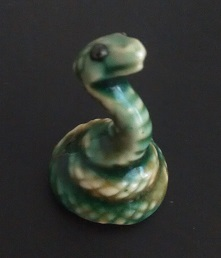
\includegraphics[scale=0.5]{ular-jpg}  
	%\caption[Ular kecil]{Ular kecil} 
	%\label{fig:ularjpg} 
%\end{figure} 
%\kant[17-19]
%
%\begin{figure}[h] 
	%\centering  
	%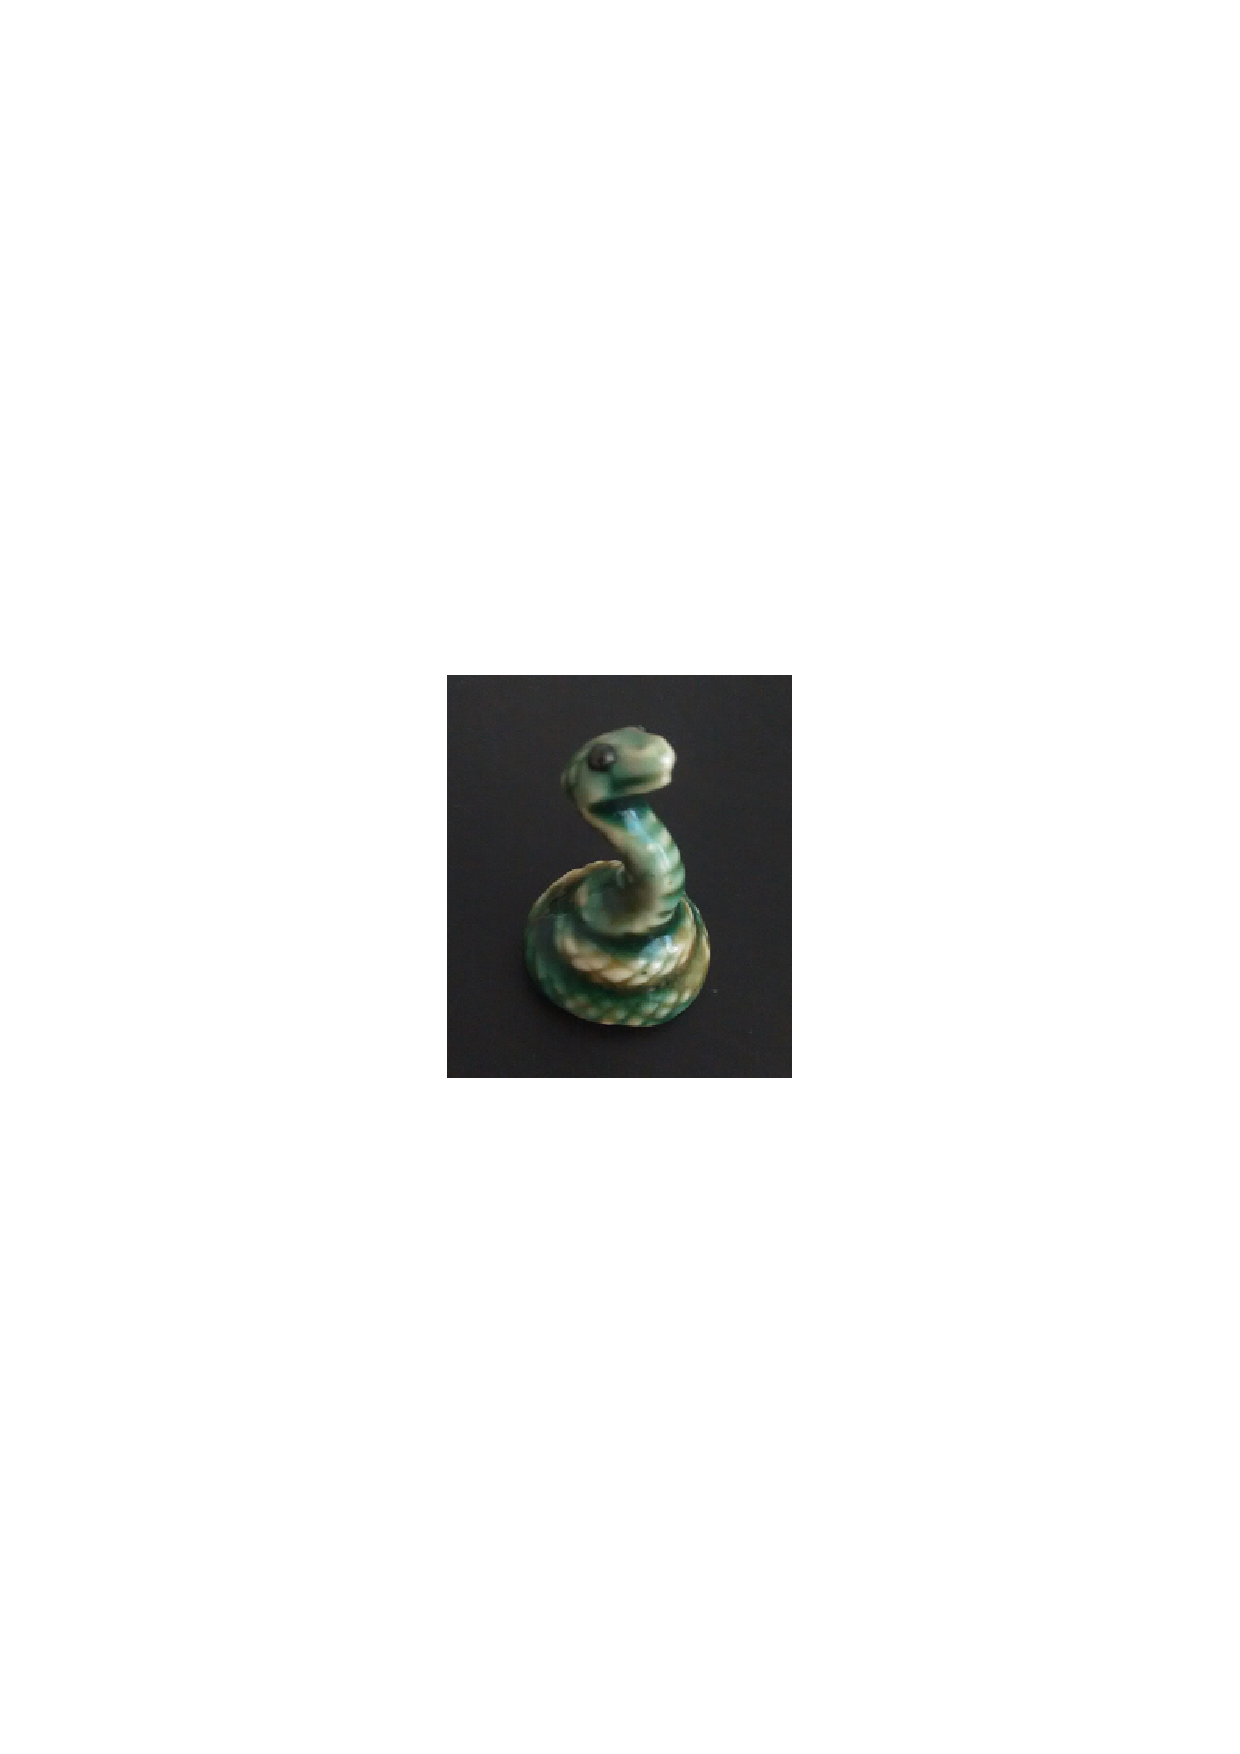
\includegraphics[scale=1]{ular-pdf}  
	%\caption[ {\it Serpentes} betina]{ {\it Serpentes} jantan} 
	%\label{fig:ularpdf} 
%\end{figure} 
 %
